\documentclass{article}
    \author{杨铭\\5130379022}
    \title{计算机视觉 - 傅里叶小波变换}
\usepackage{ctex}
\usepackage{graphicx}
\usepackage{color}
\usepackage{listings}
\usepackage{amsmath}
\usepackage{xcolor}
\usepackage[colorlinks,
            linkcolor=black,
            citecolor=green
            ]{hyperref}
\begin{document}
    \maketitle
    \tableofcontents
    \section{简述}
    \paragraph{}
    使用opencv3.0+python进行了傅里叶变换应用在图片的实验,根据网上资料,自己实现了一个优化的dft(傅里叶变换)方法。
    \section{傅里叶函数变换}
    \paragraph{三角型到复数型}
        \subparagraph{}
        三角形式的傅里叶级数:
        \begin{equation}
        f(x)=\frac{a_0}{2}+\sum_{n=1}^{\infty}(a_n\cos nx+b_n\sin nx)
        \end{equation}
        著名的欧拉公式将复数和三角函数结合在了一起:
        \begin{equation}
        e^{ix}=\cos x + i\sin x \\
        \end{equation}
        \begin{equation}
        \sin x = \frac{e^{ix}-e^{-ix}}{2i}
        \end{equation}
        \begin{equation}
        \cos x = \frac{e^{ix}+e^{-ix}}{2}
        \end{equation}
        将(3)(4)带入(1)中得到傅里叶级数的复数形式:
        \begin{align}
        f(x) & =  \frac{a_0}{2}+\sum_{n=1}^{\infty}(\frac{a_n}{2}(e^{ix}+e^{-ix})-i\frac{b_n}{2}(e^{ix}-e^{-ix}))\\
             & =  \frac{a_0}{2}+\sum_{n=1}^{\infty}(\frac{a_n-ib_n}{2}e^{ix}+\frac{a_n+ib_n}{2}e^{-ix})
        \end{align}
        其中$x=n\omega t$\\
        令$C_0=\frac{a_0}{2}$, $C_n=\frac{a_n-ib_n}{2}$, $C_{-n}=\frac{a_n+ib_n}{2}$ (n=1,2,3......)\\
        则(6)式可化简为:\\
        \begin{align}
        f(x) & = \sum_{n=-\infty}^{\infty}C_ne^{ix} \\
             & = \int_{-\infty}^{\infty}F(u)e^{iux}du
        \end{align}
        即为傅里叶级数的复数形式
    \section{DFT的实现和使用}
    \paragraph{原理分析}
        对一张图使用傅里叶变换就是将它分解成正弦和余弦波组合的形式,也就是将图片从空间域转换到频率域。二维图像的傅里叶变换可以用一下数学公式表述:
        \begin{equation}
            F(k,l)=\sum_{i=0}^{M-1}\sum_{j=0}^{N-1}f(i,j)e^{-i2\pi(\frac{k_{i}}{M}+\frac{l_{j}}{N})}
        \end{equation}
        变换后的图片每个像素包含实部和虚部两部分信息,可以计算出幅度图像来保存图像的大部分几何信息
        \begin{equation*}
        M = \sqrt{Re(DFT(I))^2+Im(DFT(I))^2}
        \end{equation*}
        参见知乎的一篇文章和班里同学姜政的讲解,对傅里叶变换进行了优化,使用矩阵乘法把时间复杂度降低到了$O(n^2)$\\
        此外我还使用了opencv2的dft和idft测试了傅里叶变换,跟我实现的效果基本一致。在进行idft之前,先使用䦢一个HPF对图片进行高通滤波,再经过idft返回原图
         \begin{figure}[htbp]
                \begin{minipage}[t]{1\linewidth}\centering
                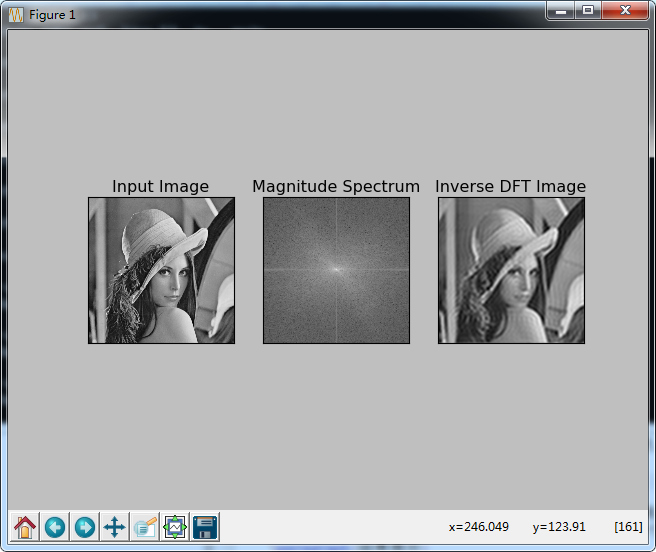
\includegraphics[width=8cm]{result.png}
                \caption{结果图}\label{1-a}
                \end{minipage}
        \end{figure}
    \section{小波变换学习}
        \subsection{简述}
        \paragraph{简述}傅里叶变换是对图片进行的整体分析变换,有其局限性。而小波变换突破了傅里叶变换的这个局限性,又可以覆盖整个图片,小波不仅在频率上是变化的,在位置上也是变化的。
        \paragraph{定义}小波是指由基本小波函数进行伸缩或位移变换得到的一系列函数波形。基本小波是具有特殊性质的实值函数,它是震荡衰减的,而且衰减的很快。可能表现为在一段定义域上有值,而在其他范围内为0。小波的局部性特征决定了它在灵活度上优于傅里叶变换
        \subsection{Haar变换}
        \paragraph{}
        Haar基本小波函数定义在[0,1]上
        \begin{figure}[htbp!]
                \begin{minipage}[t]{1\linewidth}\centering
                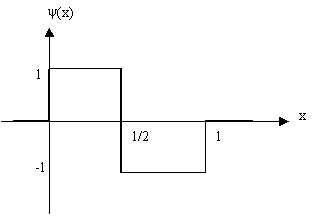
\includegraphics[width=4cm]{haar.png}
                \caption{Haar}\label{1-a}
                \end{minipage}
        \end{figure}
        \begin{equation*}
            \Psi(t)=
            \begin{cases}
            1 &\mbox{$t \in [0,0.5)$}\\
            -1 &\mbox{$t \in [0.5,1)$}
            \end{cases}
        \end{equation*}
        \paragraph{离散小波变换(DWT)}
        由于计算机中的数据都是离散的,所以要对小波变换的尺度因子、位移因子进行离散化,一般采用如下离散方式:\\
        如使用Haar作为小波因子,取尺度因子$a=a_{0}^{m},b=ka_{0}^{n}b_{0}$
        设小波基函数$\Psi(x)$为haar函数,变换函数$h_{m,n}(x)=\frac{1}{\sqrt{a_{0}^{m}}}h(\frac{1}{a_{0}^{m}}x-nb)$
        通常采用$a_0=2,b_0=1$构成离散二进小波(以二的因子伸缩和位移)
        \begin{equation*}
        h_{m,n}(x)=\frac{1}{\sqrt{2^{m}}}h(\frac{1}{2^{m}}x-n)
        \end{equation*}
        \subsection{与傅里叶变换对比}
        \begin{enumerate}
          \item 傅里叶变换描述的是整个时段内频率的特征,没有时效性,而小波变换可以做到时频分析
          \item 傅里叶变换必须采集整个图像的数据,而小波变换不需要
        \end{enumerate}
    \clearpage
       \begin{thebibliography}{90}
       {
       \bibitem{} zhipeng hu,\href{https://www.zhihu.com/question/27358117}{离散二维傅里叶变换python代码?},{\it 知乎论坛,}
       \bibitem{} 清华大学计算机科学与技术系,\href{http://media.cs.tsinghua.edu.cn/~ahz/digitalimageprocess/chapter12/chapt12_ahz.htm}{小波变换}, {\it 清华大学, } }
       \end{thebibliography}
\end{document}
